\chapter{Mathematical Formulations for Optimization and Evaluation}
\section{Optimization \& Inversion Framework}\label{app:optimization_math}
The two-step inversion process for conditioning the 3-facies generative models is mathematically defined by consecutive optimization phases: Latent Space Optimization followed by Pivotal Tuning.

\subsection{Latent Space Optimization}
During the initial Latent Space Optimization, the internal weights of the generator $G$ are frozen. Gradient descent is utilized to iteratively search the latent space $\mathcal{Z}$ for an optimal latent noise vector $\mathbf{z}^*$ that minimizes the loss between the generated facies and the true geological observations. 

Rather than evaluating the penalty exclusively at the exact well coordinates, a spatially weighted context mask is applied to enforce localized geological alignment without over-constraining the broader, unobserved reservoir architecture. A spatial influence radius is established around each well point, governed by a distance threshold ($\sigma$). This threshold acts as the standard deviation for a continuous Gaussian decay function, dictating the geostatistical \say{reach} of the well data.

Because fluvial-deltaic depositional systems are highly anisotropic—characterized by extensive horizontal continuity and limited vertical thickness—an anisotropic distance metric $d_A(v)$ is utilized, penalizing vertical deviations significantly more than horizontal ones. For any voxel $v$ in the 3D grid $\mathcal{V}$, the spatial weight mask $M(v)$ is defined as:
\begin{equation}\label{eq:spatial_mask}
    M(v) = 
    \begin{cases} 
        \exp\left(-\frac{d_A(v)^2}{2\sigma^2}\right), & \text{if } d_A(v) \leq 3\sigma \\
        0, & \text{if } d_A(v) > 3\sigma 
    \end{cases}
\end{equation}
While the threshold ($\sigma$) controls the smooth, continuous spread of the penalty, calculating gradients for distant voxels is computationally inefficient. Therefore, the mask is explicitly truncated to zero at a hard computational cutoff of $3\sigma$, where the gradient contribution becomes mathematically negligible.

The objective function is thus defined as a spatially masked Context Loss, replacing the point-wise evaluation. It is evaluated over the grid volume $\mathcal{V}$ and the $C$ total facies classes:
\begin{equation}\label{eq:latent_opt}
    \mathbf{z}^* = \arg\min_{\mathbf{z}} \left[ \sum_{v \in \mathcal{V}} \sum_{i=1}^{C} M(v) \cdot \mathcal{L}_{CE}(p_{v,i}, y_{v,i}) \right]
\end{equation}
where $\mathcal{L}_{CE}$ is the Categorical Cross-Entropy. Specifically, $y_{v,i}$ is the binary truth value (0 or 1) indicating whether class $i$ is the correct broadcasted facies for voxel $v$ (based on the nearest well data point), and $p_{v,i}$ is the generator's predicted probability for that class.

\begin{figure}[htbp!]
    \centering
    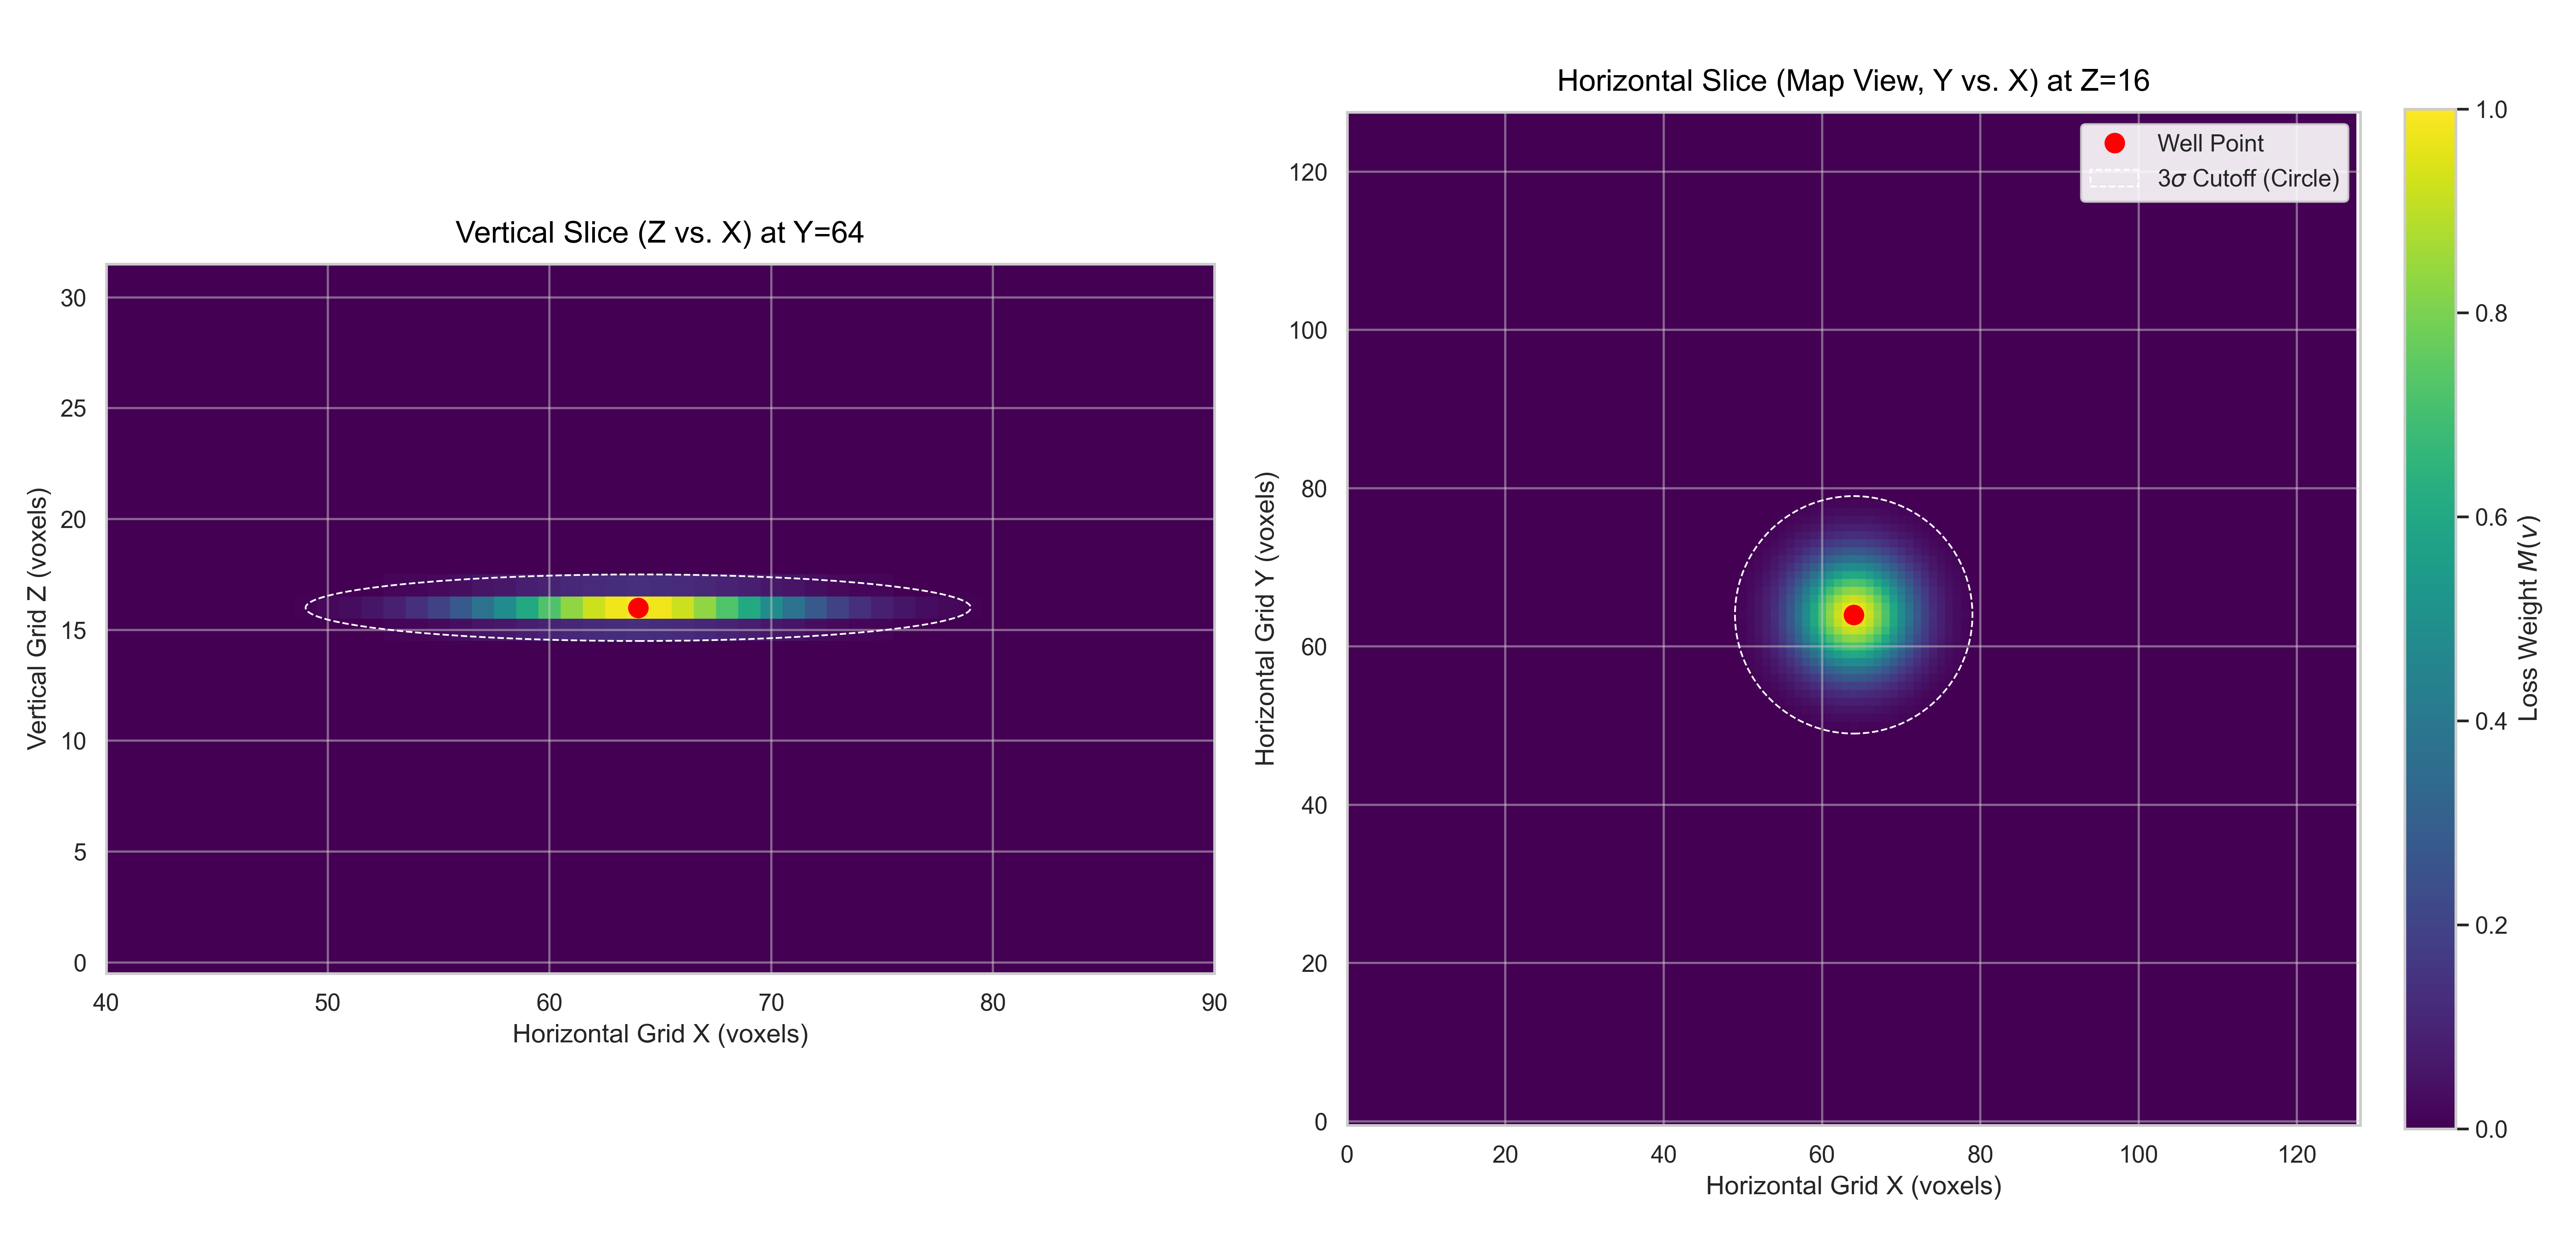
\includegraphics[width=1.0\textwidth]{figures/appendix/Appendix_C/3D_anisotropic_gaussian_mask.png}
    \caption{Orthogonal cross-sections illustrating the 3D anisotropic Gaussian weight mask $M(v)$ applied during Latent Space Optimization. The anisotropy factors are 10,1,1. The distance threshold ($\sigma$) controls the smooth spatial decay of the penalty away from the well point (red dot). Due to the anisotropic scaling factor, the mask forms a horizontal lens in the vertical cross-section (left), respecting stratigraphic deposition, while maintaining a perfectly radial spread in the map view (right). The gradient is safely truncated at a $3\sigma$ limit (dashed line) to preserve computational efficiency.}
    \label{fig:anisotropic_mask_appendix}
\end{figure}

\textbf{Computational Scaling:} Latent optimization is highly efficient. The computational cost scales linearly, $\mathcal{O}(N_{w} \cdot C)$, with the number of conditioning points $N_{w}$ and facies classes $C$. Because the network weights are frozen, the gradient is only computed with respect to the latent vector $\mathbf{z}$ (typically of dimension 512 or 1024), making this phase fast and highly scalable to dense well configurations.
\pagebreak
\subsection{Pivotal Tuning}
To overcome the inherent boundaries of the learned latent space, Pivotal Tuning~\parencite{roich2022pivotal} is applied. Using the previously optimized $\mathbf{z}^*$ as a static anchor, the generator's internal weights $\theta$ are unfrozen and optimized:
\begin{equation}\label{eq:pivotal}
    \theta^* = \arg\min_{\theta} \mathcal{L}_{CE}(G_\theta(\mathbf{z}^*)_{\text{well}}, \mathbf{y}_{\text{well}}) + \lambda ||\theta - \theta_0||_2
\end{equation}
This formulation pushes the localized outputs to perfectly match the hard conditioning data. The critical addition here is the $L_2$ regularization term $\lambda ||\theta - \theta_0||_2$, where $\theta_0$ represents the original pre-trained weights and $\lambda$ is a penalty coefficient. This term forces the modified weights to stay as close as possible to their original state, preserving the global geological realism of the model and preventing catastrophic forgetting.

\textbf{Computational Scaling:} Unlike latent optimization, Pivotal Tuning is computationally intensive. The optimization scales with the total number of trainable parameters in the generator, $|\theta|$, which often numbers in the tens of millions for 3D generative networks, $\mathcal{O}(|\theta| \cdot N_{w})$. It requires backpropagation through the entire network architecture for every iteration, scaling linearly with the size of the 3D grid output during the forward pass.


\section{Generative Evaluation Metrics}\label{app:evaluation_math}
The evaluation framework relies on advanced statistical divergence and optimal transport metrics to overcome the limitations of standard voxel-by-voxel assessments in unconditioned 3D modeling.

\subsection{Wasserstein Distance and Mean Sliced Wasserstein Distance}
The conceptual foundation for structural evaluation is the Wasserstein distance, which quantifies the optimal transport cost required to reconfigure the generated probability distribution $P_g$ into the reference real data distribution $P_r$ \parencite{panaretos2019statistical, rongier2025atowards}. It is defined as:
\begin{equation}\label{eq:wasserstein}
    \mathcal{W}(P_r, P_g) = \inf_{\gamma \sim \Pi(P_r, P_g)} \mathbb{E}_{(x,y) \sim \gamma} [\|x - y\|]
\end{equation}
where $\Pi(P_r, P_g)$ denotes the set of all joint probability distributions $\gamma(x,y)$ whose marginals are $P_r$ and $P_g$ respectively. 

Because computing Equation \ref{eq:wasserstein} over high-dimensional 3D grids suffers from the curse of dimensionality, we employ the Mean Sliced Wasserstein Distance (MSWD). MSWD projects the complex 3D distributions onto 1D lines where the optimal transport problem has a trivial, closed-form solution (sorting). Mathematically, it is defined by integrating the 1D Wasserstein distances over the unit hypersphere $\mathbb{S}^{d-1}$:
\begin{equation}\label{eq:mswd}
    \text{MSWD}(P_r, P_g) = \int_{\mathbb{S}^{d-1}} \mathcal{W}_{1D}(\mathcal{R}_{\omega} \# P_r, \mathcal{R}_{\omega} \# P_g) d\omega
\end{equation}
where $\mathcal{R}_{\omega} \# P$ denotes the projection (Radon transform) of distribution $P$ onto a 1D line defined by the direction vector $\omega$. In practice, this integral is approximated using a Monte Carlo approach by averaging over a large number of random projection angles $L$.

\textbf{Computational Scaling:} Computing the exact Wasserstein distance scales at roughly $\mathcal{O}(V^3 \log V)$, where $V$ is the total number of voxels in the 3D grid. This is intractable for standard geomodels. MSWD circumvents this by scaling at $\mathcal{O}(L \cdot V \log V)$, where $L$ is the number of projection slices. Since sorting 1D arrays is exceptionally fast, MSWD allows for robust structural comparison of massive 3D grids in a fraction of the time.

\subsection{Uncertainty and Spatial Divergence Metrics}
To assess spatial uncertainty and validate generation diversity across an ensemble, Normalized Shannon's Entropy~\parencite{shannon1948mathematical} is calculated independently for every spatial coordinate (voxel) $\mathbf{v} \in \mathbb{R}^3$. It scales the standard entropy equation by the number of geological classes ($k$) to bound the metric between 0 and 1:
\begin{equation}\label{eq:entropy_pixel}
    H_{norm}(\mathbf{v}) = -\frac{1}{\log_2(k)} \sum_{i=1}^{k} P(F_i | \mathbf{v}) \log_2 P(F_i | \mathbf{v})
\end{equation}
Here, $P(F_i | \mathbf{v})$ is the empirical probability of generating facies $F_i$ at the specific voxel $\mathbf{v}$ across the entire ensemble of realizations. An $H_{norm}(\mathbf{v})$ of $0$ implies total certainty (uniformity or potential mode collapse at that pixel), while $1$ implies total uncertainty (maximum diversity across all $k$ facies).

\textbf{Computational Scaling:} Entropy calculations are highly efficient parallel operations. The scaling is purely linear, $\mathcal{O}(V \cdot k)$, where $V$ is the total number of voxels, making it perfectly suited for massive 3D grids regardless of ensemble size.

To quantify the distributional disagreement between the true reference models ($P$) and the generated models ($Q$), we calculate the pixel-wise Kullback-Leibler (KL) divergence~\parencite{kullback1951information}:
\begin{equation}\label{eq:kl_div_pixel}
    D_{KL}(P_{\mathbf{v}} \parallel Q_{\mathbf{v}}) = \sum_{i=1}^{k} P(F_i | \mathbf{v}) \log_2\left(\frac{P(F_i | \mathbf{v})}{Q(F_i | \mathbf{v})}\right)
\end{equation}
Because KL divergence is asymmetric and unbounded, it is transformed into the Jensen-Shannon (JS) divergence \parencite{lin1991divergence} to provide a bounded, symmetric measure of stochastic spread at each voxel:
\begin{equation}\label{eq:js_div_pixel}
    D_{JS}(\mathbf{v}) = \frac{1}{2} D_{KL}(P_{\mathbf{v}} \parallel M_{\mathbf{v}}) + \frac{1}{2} D_{KL}(Q_{\mathbf{v}} \parallel M_{\mathbf{v}}) 
\end{equation}
where $M_{\mathbf{v}} = \frac{1}{2}(P_{\mathbf{v}} + Q_{\mathbf{v}})$ is the mixture distribution at voxel $\mathbf{v}$. 

Finally, to aggregate this 3D grid of spatial conflict into a single definitive scalar for model evaluation, the mean JS divergence is computed across the entire spatial volume $\mathcal{V}$:
\begin{equation}\label{eq:js_div_scalar}
    \overline{D}_{JS} = \frac{1}{|\mathcal{V}|} \sum_{\mathbf{v} \in \mathcal{V}} D_{JS}(\mathbf{v})
\end{equation}

\textbf{Computational Scaling:} Similar to entropy, JS Divergence operates strictly on the pre-computed probability mass functions of the respective ensembles. Therefore, the scalar aggregation scales linearly with the number of voxels evaluated, $\mathcal{O}(V)$. It remains computationally trivial even for massive, high-resolution spatial domains.

To aggregate this spatial conflict into a single quantitative scalar comparing two datasets, we utilize the Jensen-Shannon (JS) divergence \parencite{lin1991divergence}. It measures the symmetric stochastic spread between the true reference distributions ($P$) and the generated distributions ($Q$):
\begin{equation}\label{eq:js_div}
    D_{JS}(P \parallel Q) = \frac{1}{2} D_{KL}(P \parallel M) + \frac{1}{2} D_{KL}(Q \parallel M) 
\end{equation}
where $M = \frac{1}{2}(P + Q)$ is a mixture distribution, and $D_{KL}$ is the standard Kullback-Leibler divergence~\parencite{kullback1951information}, explicitly formulated as:
\begin{equation}\label{eq:kl_div}
    D_{KL}(P \parallel Q) = \sum_{x} P(x) \log\left(\frac{P(x)}{Q(x)}\right)
\end{equation}
Unlike $D_{KL}$, which is asymmetric and can approach infinity if $Q(x)$ is zero, $D_{JS}$ is strictly symmetric ($D_{JS}(P \parallel Q) = D_{JS}(Q \parallel P)$) and bounded between $[0, 1]$ when calculated with base-2 logarithms, making it a robust final scalar for spatial fidelity.

\textbf{Computational Scaling:} Similar to entropy, JS Divergence operates strictly on the pre-computed probability mass functions of the respective ensembles. Therefore, it scales linearly with the number of spatial bins/voxels evaluated, $\mathcal{O}(V)$. It remains computationally trivial even for massive, high-resolution spatial domains.